\newif\ifshowsolutions
\showsolutionstrue
\documentclass{article}
\usepackage{listings}
\usepackage{amsmath}
\usepackage{subfig}
\usepackage{amsthm}
\usepackage{amsmath}
\usepackage{amssymb}
\usepackage{graphicx}
\usepackage{mdwlist}
\usepackage{geometry}
\usepackage{titlesec}
\usepackage{palatino}
\usepackage{mathrsfs}
\usepackage{fancyhdr}
\usepackage{paralist}
\usepackage{todonotes}
\usepackage{tikz}
\usepackage{float} % Place figures where you ACTUALLY want it
\usepackage{comment} % A hack to toggle sections
\usepackage{ifthen}
\usepackage{mdframed}
\usepackage{verbatim}
\usepackage{listings}
\usepackage{bbm}
\usepackage{upquote} % Prevents backticks replacing single-quotes in verbatim
\usepackage[strings]{underscore}
\usepackage[colorlinks=true]{hyperref}
\usetikzlibrary{positioning,shapes,backgrounds}

\geometry{margin=1in}
\geometry{headheight=2in}
\geometry{top=2in}

\setlength{\marginparwidth}{2.15cm}
\setlength{\parindent}{0em}
\setlength{\parskip}{0.6\baselineskip}

\rhead{}
\lhead{}

% Spacing settings.
\titlespacing\section{0pt}{12pt plus 2pt minus 2pt}{0pt plus 2pt minus 2pt}
\titlespacing\subsection{0pt}{12pt plus 4pt minus 2pt}{0pt plus 2pt minus 2pt}
\titlespacing\subsubsection{0pt}{12pt plus 4pt minus 2pt}{0pt plus 2pt minus 2pt}
\renewcommand{\baselinestretch}{1.15}

% Shortcuts for commonly used operators.
\newcommand{\E}{\mathbb{E}}
\newcommand{\Var}{\operatorname{Var}}
\newcommand{\Cov}{\operatorname{Cov}}
\newcommand{\Bias}{\operatorname{Bias}}
\DeclareMathOperator{\argmin}{arg\,min}
\DeclareMathOperator{\argmax}{arg\,max}

% Do not number subsections and below.
\setcounter{secnumdepth}{1}

% Custom format subsection.
\titleformat*{\subsection}{\large\bfseries}

% Set up the problem environment.
\newcounter{problem}[section]
\newenvironment{problem}[1][]
  {\begingroup
    \setlength{\parskip}{0em}
    \refstepcounter{problem}\par\addvspace{1em}\textbf{Problem~\Alph{problem}\!
    \ifthenelse{\equal{#1}{}}{}{ [#1 points]}:}
  \endgroup}

% Set up the subproblem environment.
\newcounter{subproblem}[problem]
\newenvironment{subproblem}[1][]
  {\begingroup
    \setlength{\parskip}{0em}
    \refstepcounter{subproblem}\par\medskip\textbf{\roman{subproblem}.\!
    \ifthenelse{\equal{#1}{}}{}{ [#1 points]:}}
  \endgroup}

% Set up the teachers and materials commands.
\newcommand\teachers[1]
  {\begingroup
    \setlength{\parskip}{0em}
    \vspace{0.3em} \textit{\hspace*{2em} TAs responsible: #1} \par
  \endgroup}
\newcommand\materials[1]
  {\begingroup
    \setlength{\parskip}{0em}
    \textit{\hspace*{2em} Relevant materials: #1} \par \vspace{1em}
  \endgroup}

% Set up the hint environment.
\newenvironment{hint}[1][]
  {\begin{em}\textbf{Hint: }}
  {\end{em}}


% Set up the solution environment.
\ifshowsolutions
  \newenvironment{solution}[1][]
    {\par\medskip \begin{mdframed}\textbf{Solution~\Alph{problem}#1:} \begin{em}}
    {\end{em}\medskip\end{mdframed}\medskip}
  \newenvironment{subsolution}[1][]
    {\par\medskip \begin{mdframed}\textbf{Solution~\Alph{problem}#1.\roman{subproblem}:} \begin{em}}
    {\end{em}\medskip\end{mdframed}\medskip}
\else
  \excludecomment{solution}
  \excludecomment{subsolution}
\fi




%%%%%%%%%%%%%%%%%%%%%%%%%%%%%%
% HEADER
%%%%%%%%%%%%%%%%%%%%%%%%%%%%%%

\chead{%
  {\vbox{%
      \vspace{2mm}
      \large
      Machine Learning \& Data Mining \hfill
      Caltech CS/CNS/EE 155 \hfill \\[1pt]
      Homework 6\hfill
      February 2022 \\
    }
  }
}

\begin{document}
\pagestyle{fancy}

%%%%%%%%%%%%%%%%%%%%%%%%%%%%%%
% POLICIES
%%%%%%%%%%%%%%%%%%%%%%%%%%%%%%
\section*{Policies}
\begin{itemize}
  \item \textbf{Due 9 PM, March $2^\text{nd}$}, via Gradescope.
  \item You are free to collaborate on all of the problems, subject to the collaboration policy stated in the syllabus.
  \item In this course, we will be using Google Colab for code submissions. You will need a Google account.
  \item This set uses PyTorch, a Python package for neural networks. We recommend using Google Colab, which comes with PyTorch already installed.
\end{itemize}

\section*{Submission Instructions}
\begin{itemize}
\item Submit your report as a single .pdf file to Gradescope, under "Set 6 Report". 
	\item In the report, \textbf{include any images generated by your code} along with your answers to the questions.
	\item Submit your code by \textbf{sharing a link in your report} to your Google Colab notebook for each problem (see naming instructions below). Make sure to set sharing permissions to at least "Anyone with the link can view". \textbf{Links that can not be run by TAs will not be counted as turned in.} Check your links in an incognito window before submitting to be sure. 
	\item For instructions specifically pertaining to the Gradescope submission process, see \url{https://www.gradescope.com/get_started#student-submission}.
\end{itemize}

\section*{Google Colab Instructions}
For each notebook, you need to save a copy to your drive.
\begin{enumerate}
	\item Open the github preview of the notebook, and click the icon to open the colab preview.
	\item On the colab preview, go to File $\rightarrow$ Save a copy in Drive.
	\item Edit your file name to “lastname_firstname_set_problem”, e.g.”yue_yisong_set6_prob2.ipynb”
\end{enumerate}

\newpage
%%%%%%%%%%%%%%%%%%%%%%%%%%%%%%
% PROBLEM 1
%%%%%%%%%%%%%%%%%%%%%%%%%%%%%%

\section{Class-Conditional Densities for Binary Data [25 Points, 8 EC Points]}
This problem will test your understanding of probabilistic models, especially Naive Bayes.
Consider a generative classifier for $C$ classes, with class conditional density $p(x | y)$ and a uniform class prior $p(y)$. Suppose all the $D$ features are binary, $x_j \in \{0, 1 \}$. If we assume all of the features are conditionally independent, as in Naive Bayes, we can write:
$$p(x \mid y = c) = \prod_{j=1}^D p(x_j \mid y = c) $$
This requires storing $DC$ parameters. 

Now consider a different model, which we will call the `full' model, in which all the features are fully \textit{dependent}.

\problem[9] Use the chain rule of probability to factorize $p(x \mid y)$, and let $\theta_{xjc} = p(x_j | x_{1, \ldots, j - 1}, y = c)$. Assuming we store each $\theta_{xjc}$, how many parameters are needed to represent this factorization? Use big-O notation. 

\begin{solution}
  Using the chain rule of probability:
  \begin{equation}
    p(x \mid y) = p(x_D \mid x_{1:D-1}, y = c) p(x_{D-1} \mid x_{1:D-2}, y = c) ... p(x_1 \mid y = c)
  \end{equation}
  Substituting the definition of $\theta_{xjc}$,
  \begin{equation}
    p(x \mid y) = \theta_{xDc} \theta_{x(D-1)c} ... \theta_{x1c} = \prod_{j=1}^{D} \theta_{xjc}
  \end{equation}
  Storing each $\theta_{xjc}$ requires $C*2^{j-1}$ parameters because there are two possibilities for each $x_{1:j-1}$. The sum of the geometric series $\sum_{j=1}^{D} C*2^{j-1} = C*2^D$. Thus the number of parameters needed is of order $O(C \times 2^D)$.
\end{solution}

\problem[8] Assume we did no such factorization, and just used the joint probability $p(x \mid y = c)$. How many parameters would we need to estimate in order be able to compute $p(x | y = c)$ for arbitrary $x$ and $c$? How does this compare to your answer from the previous part? Again, use big-O notation.

\begin{solution}
  Computing the joint probability distribution  $p(x \mid y = c)$ also has complexity $O(C \times 2^D)$ because there are $D$ binary features and $C$ classes, which is the same order as the previous part.
\end{solution}

\problem[4] Assume the number of features $D$ is fixed. Let there be $N$ training cases. If the sample size $N$ is very small, which model (Naive Bayes or full) is likely to give lower test set error, and why?

\begin{solution}
  When the sample size is small, Naive Bayes is likely to give a lower test set error because conditional independence is a good assumption if there are fewer samples. Learning a full model could lead to overfitting when trying to learn a relationship between different features.
\end{solution}

\problem[4] If the sample size $N$ is very large, which model (Naive Bayes or full) is likely to give lower test set error, and why?
\begin{solution} 
  When the sample size is large, the full model is likely to give a lower test error. Conditional independence is not a good assumption in this case and will lead to underfitting. Given enough data, the model should be able accurately to learn the feature dependencies on each other, which makes the full model a better choice.
\end{solution}

\problem[8 EC] Assume all the parameter estimates have been computed. What is the computational complexity of making a prediction, i.e. computing $p(y \mid x)$, using Naive Bayes for a single test case? What is the computation complexity of making a prediction with the full model? In justifying your answer for the full model, choose either the implementation in 1A or 1B and state your choice. For the full-model case, assume that converting a $D$-bit vector to an array index is an $O(D)$ operation.  Also, recall that we have assumed a uniform class prior. 

\begin{solution}
  Not attempted.
\end{solution}


\newpage
\section{Sequence Prediction [75 Points]}

In this problem, we will explore some of the various algorithms associated with Hidden Markov Models (HMMs), as discussed in lecture.
We have also uploaded a note on HMMs to the github that might be helpful.

\subsection{Sequence Prediction}

These next few problems will require extensive coding, so be sure to start early! 
\begin{itemize}
  \item You will write an implementation for the hidden Markov model in the cell for \texttt{HMM Code} in the notebook given to you, within the appropriate functions where indicated. There should be no need to write additional functions or use NumPy in your implementation, but feel free to do so if you would like.
  \item You can (and should!) use the helper cells for each of the subproblems in the notebook, namely \texttt{2A}, \texttt{2Bi}, \texttt{2Bii}, \texttt{2C}, \texttt{2D}, and \texttt{2F}. These can be used to run and check your implementations for each of the corresponding problems. The cells provide useful output in an easy-to-read format. There is no need to modify these cells.
  \item Lastly, the cell for \texttt{Utility} contains some functions used for loading data directly from the class github repository. There is no need to modify this cell. \\
\end{itemize}

The supplementary data folder of the class github repository contains 6 files titled \texttt{sequence_data0.txt}, \texttt{sequence_data1.txt}, ... , \texttt{sequence_data5.txt}. Each file specifies a \textbf{trained} HMM. The first row contains two tab-delimited numbers: the number of states $Y$ and the number of types of observations $X$ (i.e. the observations are $0, 1, . . . , X - 1$). The next $Y$ rows of $Y$ tab-delimited floating-point numbers describe the state transition matrix. Each row represents the current state, each column represents a state to transition to, and each entry represents the probability of that transition occurring. The next $Y$ rows of $X$ tab-delimited floating-point numbers describe the output emission matrix, encoded analogously to the state transition matrix. The file ends with 5 possible emissions from that HMM. \\

The supplementary data folder also contains one additional file titled \texttt{ron.txt}. This is used in problems 2C and 2D and is explained in greater detail there. 
\indent\problem[10] % indent for consistency
For each of the six trained HMMs, find the max-probability state sequence for each of the five input sequences at the end of the corresponding file. To complete this problem, you will have to implement the Viterbi algorithm (in \texttt{viterbi()} of the \texttt{HiddenMarkovModel} object). Write your implementation well, as we will be reusing it in a later problem. See the end of problem 2B for a big hint! Note that you do not need to worry about underflow in this part.

In your report, show your results on the 6 files. (Copy-pasting the results of the cell for \texttt{2A} suffices.)
\begin{solution}   
  \href{https://colab.research.google.com/drive/1Rrg0gpfLqg3G2KZZfZJjnOL_cBieTled}{Link to code}
    \begin{center}
      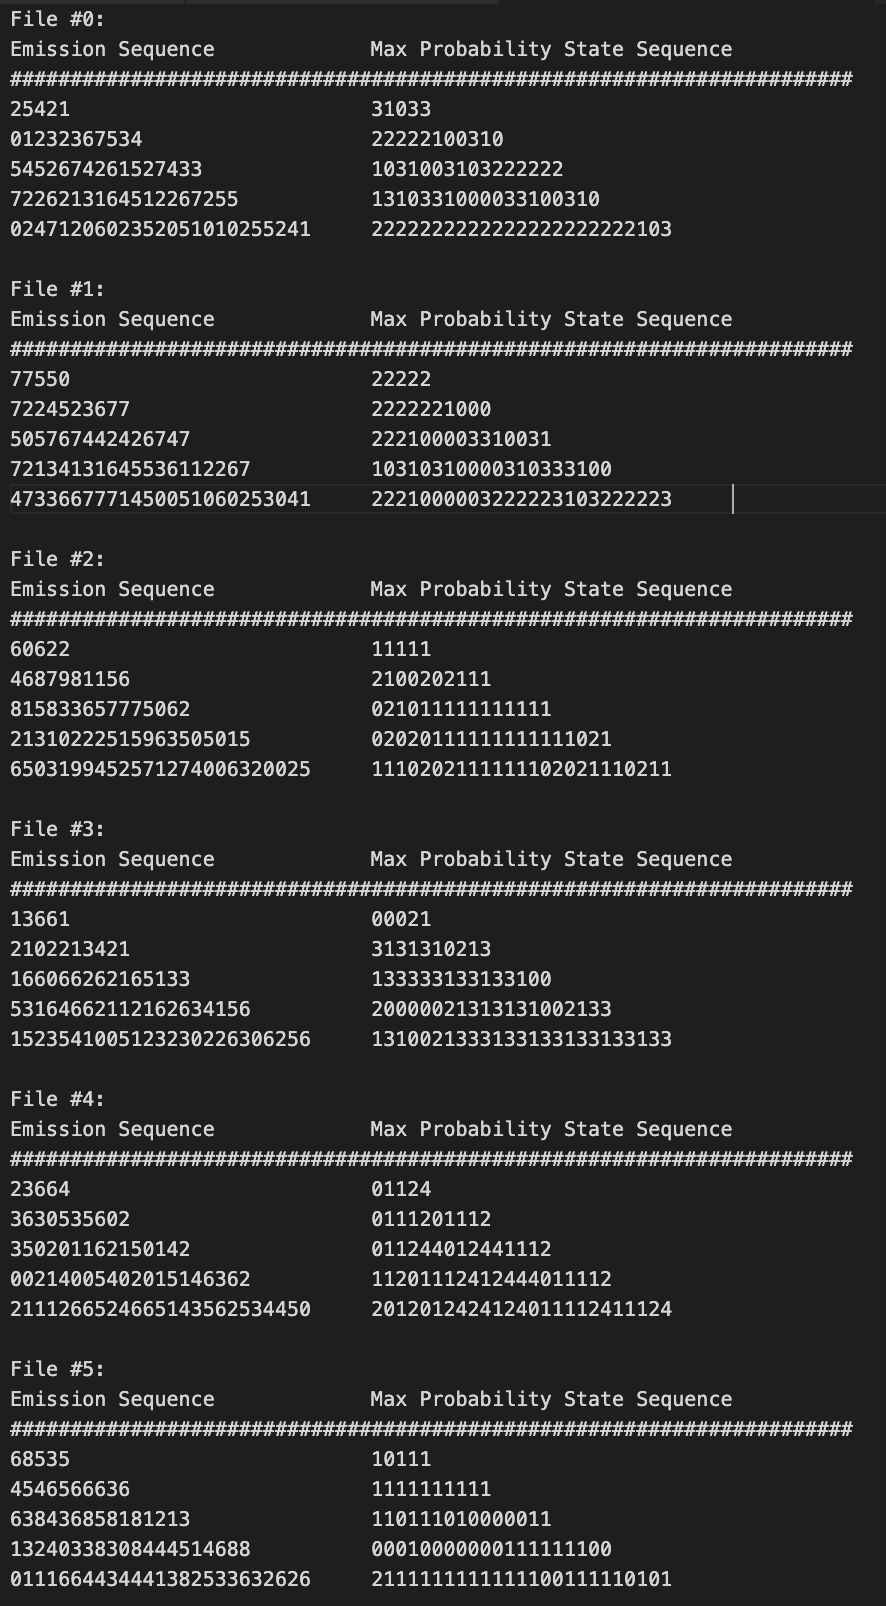
\includegraphics[width=0.6\textwidth]{prob2a.png}
    \end{center}
\end{solution}

\indent\problem[17] % indent for consistency
For each of the six trained HMMs, find the probabilities of emitting the five input sequences at the end of the corresponding file. To complete this problem, you will have to implement the Forward algorithm and the Backward algorithm. You may assume that the initial state is randomly selected along a uniform distribution (the starting state transition probabilities are defined in \texttt{self.A\_start} in \texttt{HiddenMarkovModel}). Again, write your implementation well, as we will be reusing it in a later problem. \\

Note that the probability of emitting an input sequence can be found by using either the $\alpha$ vectors from the Forward algorithm or the $\beta$ vectors from the Backward algorithm. You don't need to worry about this, as it is done for you in \texttt{probability\_alphas()} and \texttt{probability\_betas()}.

Implement the Forward algorithm. In your report, show your results on the 6 files. \\
Implement the Backward algorithm. In your report, show your results on the 6 files. \\

After you complete problems 2A and 2B, you can compare your results (the probabilities from the forward and backward algorithms should be the same) for the file titled \texttt{sequence_data0.txt} with the values given in the table below:
\begin{center}
  \begin{tabular}{ l | l |l | l }
Dataset & Emission Sequence & Max-probability State Sequence & Probability of Sequence  \\ \hline
0 & 25421                      &  31033           & 4.537e-05\\
0 & 01232367534                &  22222100310       & 1.620e-11\\
0 & 5452674261527433           &  1031003103222222      & 4.348e-15\\
0 & 7226213164512267255        &  1310331000033100310   & 4.739e-18\\
0 & 0247120602352051010255241  &  2222222222222222222222103 & 9.365e-24
 \\ \hline
 \end{tabular}
\end{center}
  
\begin{solution}
  Forward algorithm:
  \begin{center}
  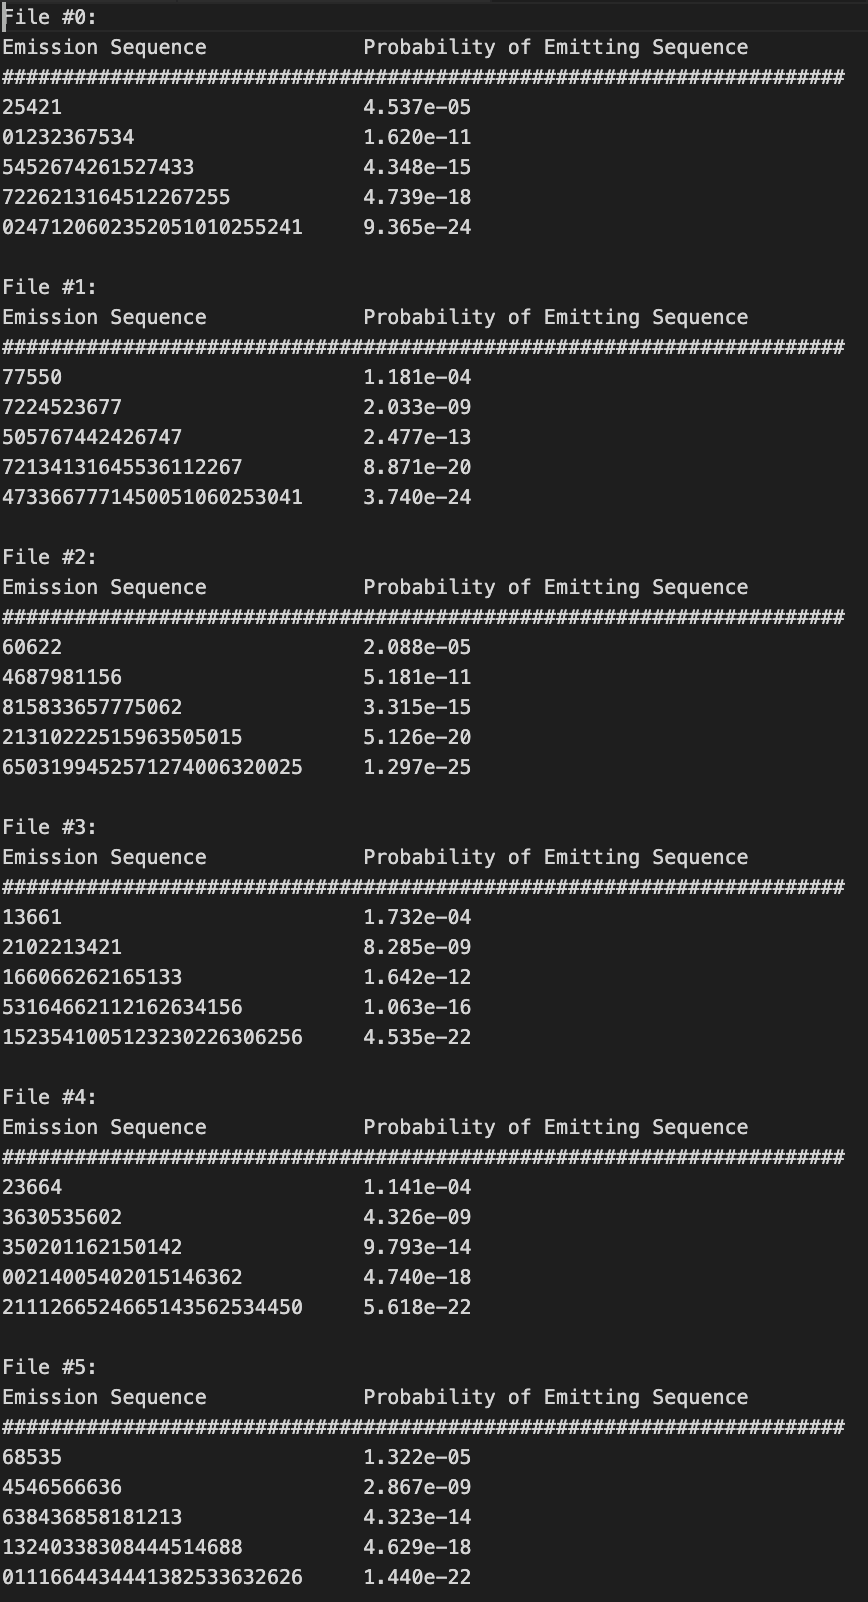
\includegraphics[width=0.6\textwidth]{prob2bi.png}
  \end{center}
  Backward algorithm:
  \begin{center}
  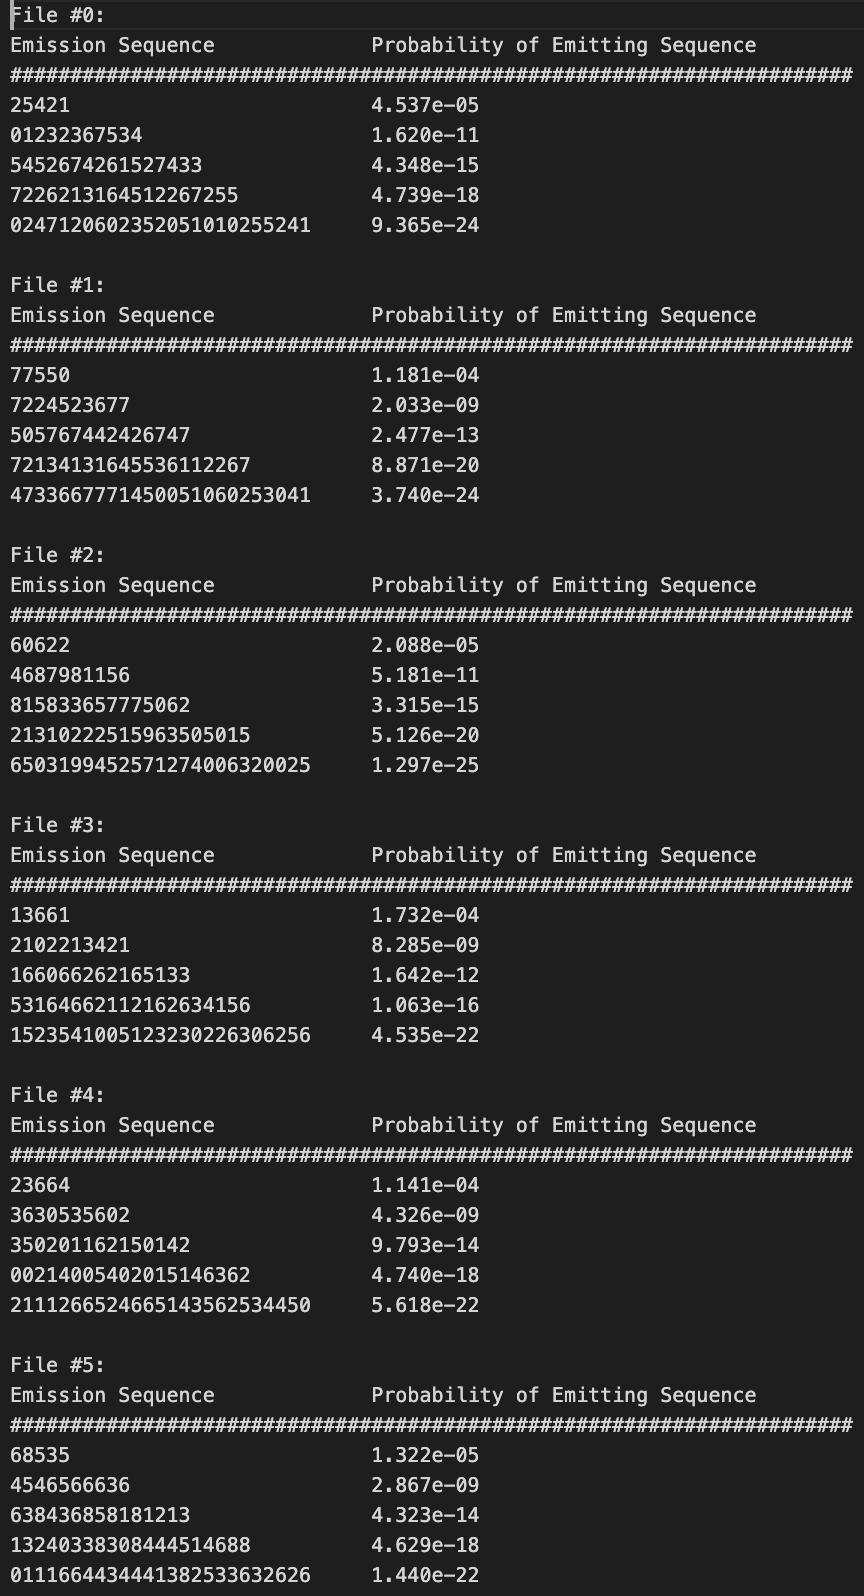
\includegraphics[width=0.6\textwidth]{prob2bii.png}
  \end{center}
\end{solution}

\subsection{HMM Training}
Ron is an avid music listener, and his genre preferences at any given time depend on his mood. Ron's possible moods are happy, mellow, sad, and angry. Ron experiences one mood per day (as humans are known to do) and chooses one of ten genres of music to listen to that day depending on his mood. \\

Ron's roommate, who is known to take to odd hobbies, is interested in how Ron's mood affects his music selection, and thus collects data on Ron's mood and music selection for six years (2190 data points). This data is contained in the supplementary file \texttt{ron.txt}. Each row contains two tab-delimited strings: Ron's mood and Ron's genre preference that day. The data is split into 12 sequences, each corresponding to half a year's worth of observations. The sequences are separated by a row containing only the character \texttt{-}.
\noindent\problem[10] % indent for consistency
Use a single M-step to train a supervised Hidden Markov Model on the data in \texttt{ron.txt}. What are the learned state transition and output emission matrices?

Tip: the \((1,1)\) entry of your transition matrix should be \verb|2.833e-01|, and the \((1,1)\) entry of your observation matrix should be \verb|1.486e-01|.
\begin{solution}
  \begin{center}
    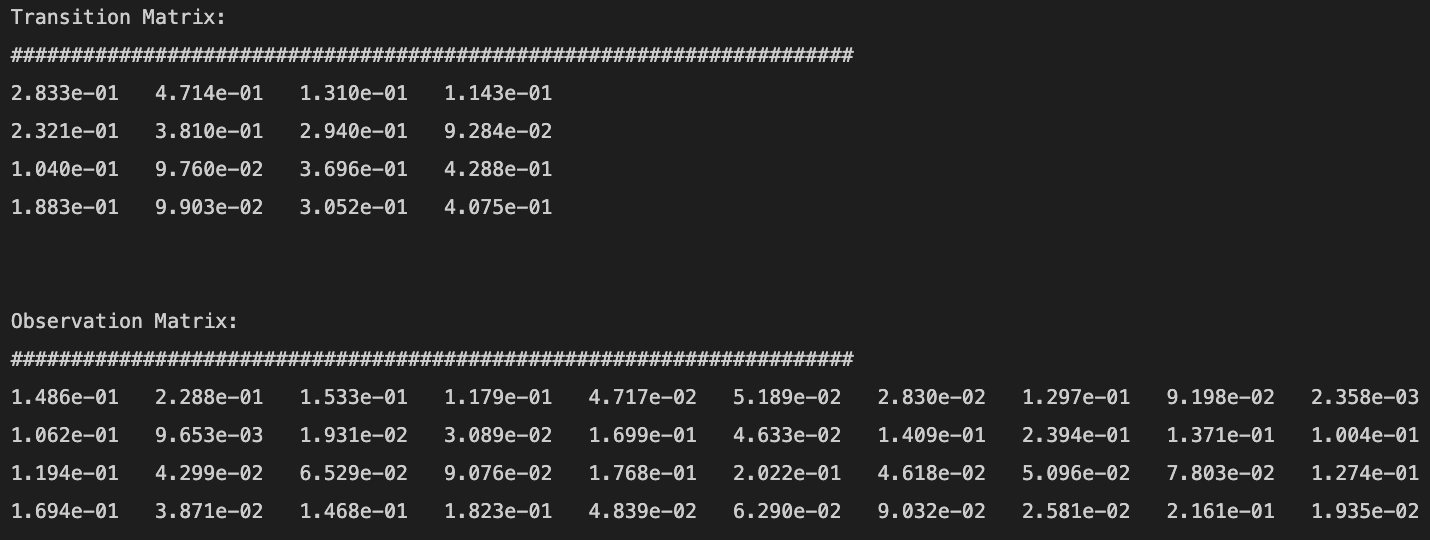
\includegraphics[width=0.9\textwidth]{prob2c.png}
  \end{center}
\end{solution}
\indent\problem[15] % indent for consistency
Now suppose that Ron has a third roommate who is also interested in how Ron's mood affects his music selection. This roommate is lazier than the other one, so he simply steals the first roommate's data. Unfortunately, he only manages to grab half the data, namely, Ron's choice of music for each of the 2190 days.

In this problem, we will train an unsupervised Hidden Markov Model on this data. Recall that unsupervised HMM training is done using the Baum-Welch algorithm and will require repeated EM steps. For this problem, we will use 4 hidden states and run the algorithm for 1000 iterations. The transition and observation matrices are initialized for you in the helper functions \texttt{supervised\_learning()} and \texttt{unsupervised\_learning()} such that they are random and normalized.

What are the learned state transition and output emission matrices? Please report the result using random seed state 1, as is done by default in the notebook.

Tips for debugging:
\begin{itemize}
  \item The rows of the state transition and output emitting matrices should sum to 1.
  \item Your matrices should not change drastically every iteration.
  \item After many iterations, your matrices should converge.
  \item If you used random seed 1 for this computation (as is done by default in the notebook), the \((1,1)\) entry of the state transition matrix should be \verb|5.075e-01|, and the \((1,1)\) entry of the output emission matrix should be \verb|1.117e-01|.
\end{itemize}

\begin{solution}
  \begin{center}
    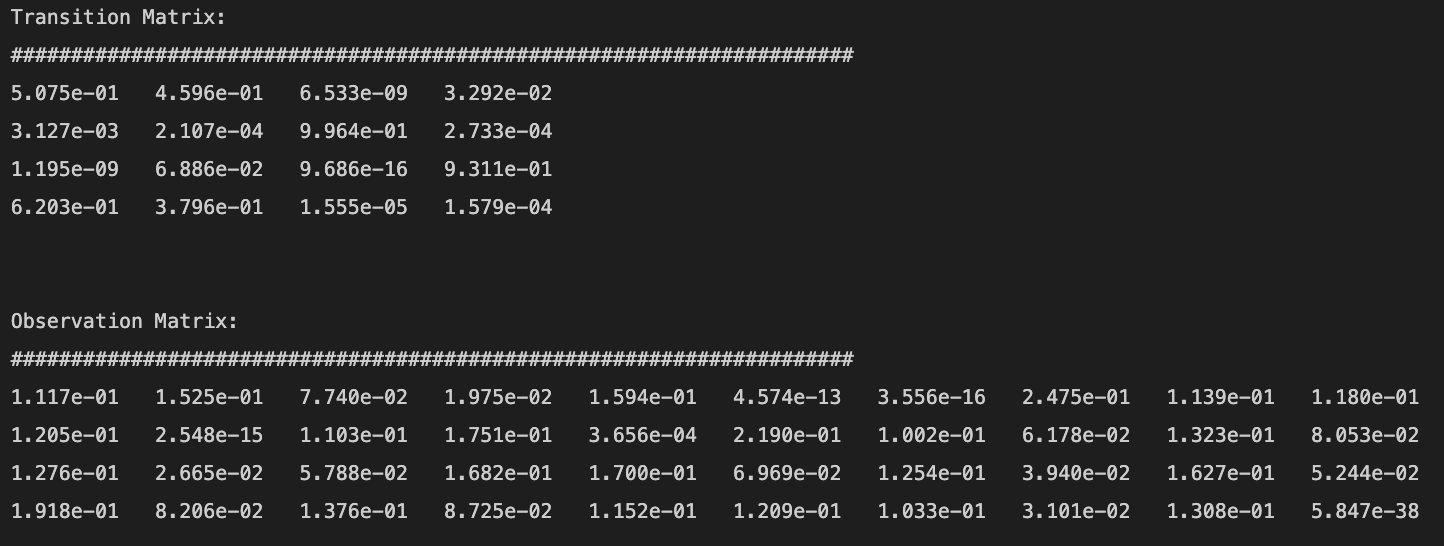
\includegraphics[width=0.9\textwidth]{prob2d.png}
  \end{center}
\end{solution}

\problem[5] How do the transition and emission matrices from 2C and 2D compare? Which do you think provides a more accurate representation of Ron's moods and how they affect his music choices? Justify your answer. Suggest one way that we may be able to improve the method (supervised or unsupervised) that you believe produces the less accurate representation. 

\begin{solution}
  The transition matrix for 2D generally has smaller values than that from 2C, which menas this matrix is more sparse. The matrices from 2C are a likely a better representation of Ron's moods because it is actually trained with the moods, which makes the transition and observation matrices optimal. However, the unsupervised method is not able to learn from these moods. We could improve the unsupervised model by providing a meaningful prior for the transition or observation matrix, based on how Ron's moods might be distributed.
\end{solution}

\subsection{Sequence Generation}
Hidden Markov Models fall under the umbrella of generative models and therefore can be used to not only predict sequential data, but also to generate it.

\problem[5] Run the cell for this problem. The code in the cell loads the trained HMMs from the files titled \texttt{sequence_data0.txt}, $\ldots$ , \texttt{sequence_data5.txt} and uses the six models to probabilistically generate five sequences of emissions from each model, each of length 20. In your report, show your results. 

\begin{solution}
  \begin{center}
    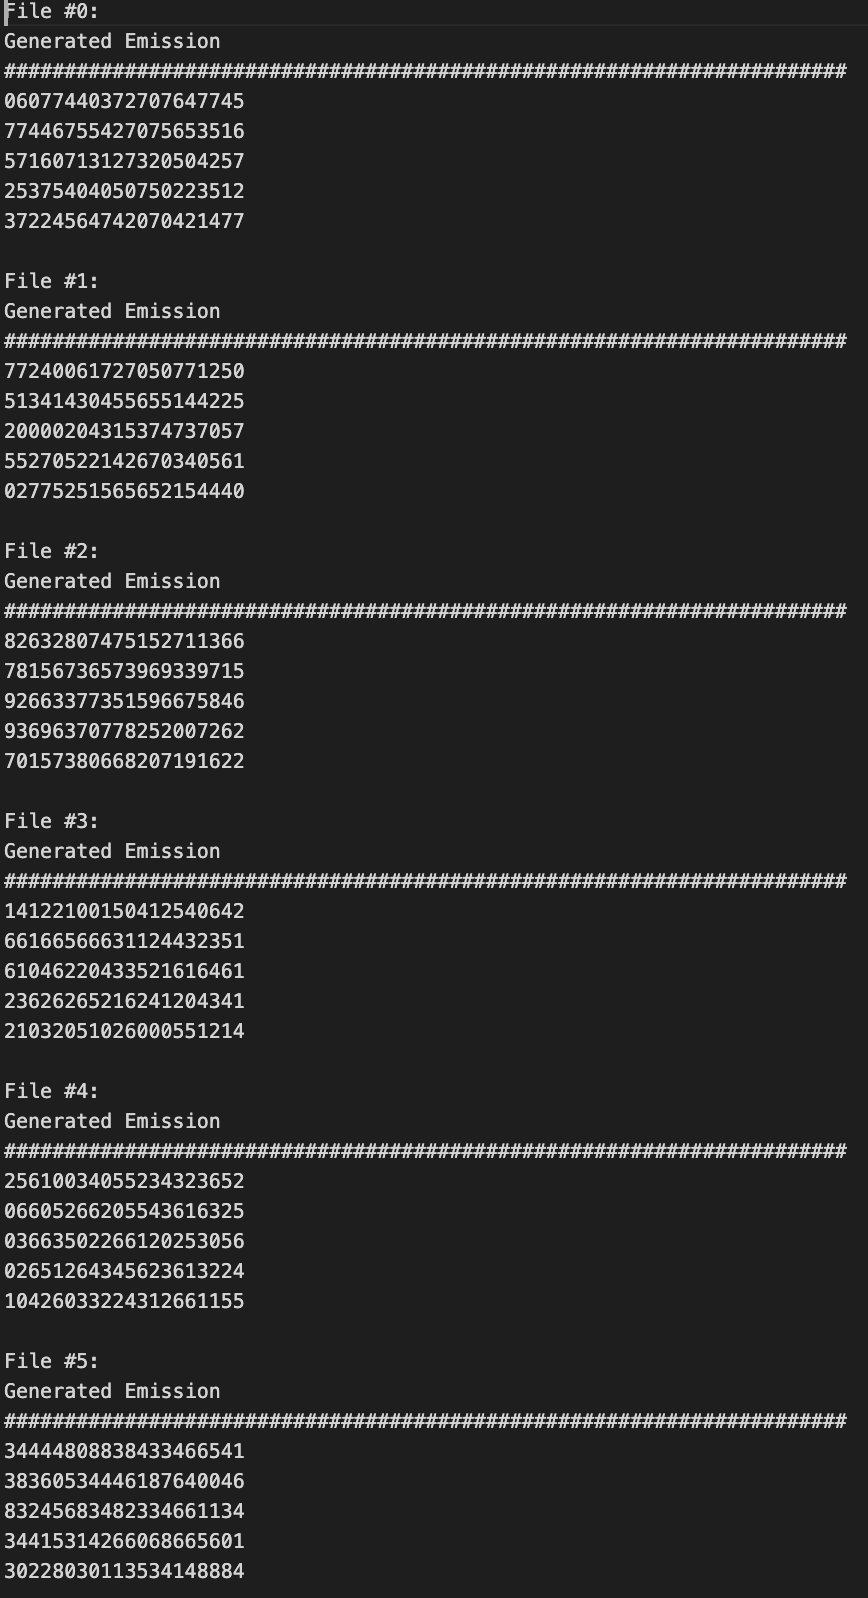
\includegraphics[width=0.40\textwidth]{prob2f.png}
  \end{center}
\end{solution}

\subsection{Visualization \& Analysis}

Once you have implemented the HMM code part of the notebook, load and run the cells for the following subproblems. Here you will apply the HMM you have implemented to the Constitution. There is no coding required for this part, only analysis.

Answer the following problems in the context of the visualizations in the notebook.

\indent\problem[3] % indent for consistency
What can you say about the sparsity of the trained $A$ and $O$ matrices? How does this sparsity affect the transition and observation behaviour at each state?
\begin{solution}
  $A$ and $O$ are both sparse matrices, but $O$ is slightly more sparse since it is larger. The sparsity of $A$ implies that very few states are likely to be achieved from a given state. The sparsity of $O$ implies that very few observations are likely to be generated from a given state.
\end{solution}

\indent\problem[5] % indent for consistency
How do the sample emission sentences from the HMM change as the number of hidden states is increased? What happens in the special case where there is only one hidden state? In general, when the number of hidden states is unknown while training an HMM for a fixed observation set, can we increase the training data likelihood by allowing more hidden states?

\begin{solution}
  As the number of hidden states is increased, the emission sentences become more and more comprehensible, and resembling sentences from the constitution. For example, one hidden state produces a nonsensical sentence: "To the and meet their extend same states to from in any the time any elected states of the by proper they the pursuance for..." but once we have 4 hidden states, the emitted sentences make more sense: "Be of established inhabitant employed and proposing to such seat provided their test faithfully at committed or no one may witnesses of three executive of..." It appears that there may be some overfitting with 16 hidden states, as the sentence is less comprehensible and more skewed to unique words in the constitution. In the special case of one hidden state, the words are basically ordered, because they have the same probability of appearing anywhere in the sentence. In general, we can fit better to the training data by allowing more hidden states because this allows for more possible associations in the $A$ and $O$ matrices, which can only help on the training set.
\end{solution}


\indent\problem[5] % indent for consistency
Pick a state that you find semantically meaningful, and analyze this state and its wordcloud. What does this state represent? How does this state differ from the other states? Back up your claim with a few key words from the wordcloud.
\begin{solution}
  State 3 is semantically meaningful from a grammatical standpoint. While many of the other states are grouped around a certain concept, state 3 seems to be grouped around comparison words. "two," "three," and "every" are the most important words in this state in addition to other numbers and comparison words such as "different."
\end{solution}



\end{document}
